\documentclass{beamer}
\usetheme{metropolis}

\usepackage{amssymb, amsmath}
\usepackage[utf8]{inputenc}
\usepackage{babel}
\usepackage[T1]{fontenc}
\usepackage[autostyle=true]{csquotes}
\usepackage[sfdefault]{FiraSans}
\usepackage{hyperref}

\newcommand{\red}[1]{\textcolor{red}{#1}}
\newcommand{\blue}[1]{\textcolor{blue}{#1}}

\newcommand{\del}[1]{\mathbf{\nabla #1}}

\DeclareMathOperator{\tr}{tr} 

%\setbeamertemplate{caption}{\raggedright\insertcaption\par} 
\setbeamertemplate{bibliography item}{\insertbiblabel}

\newcommand{\backupbegin}{
   \newcounter{framenumberappendix}
   \setcounter{framenumberappendix}{\value{framenumber}}
}
\newcommand{\backupend}{
   \addtocounter{framenumberappendix}{-\value{framenumber}}
   \addtocounter{framenumber}{\value{framenumberappendix}} 
}

\title[Corner Region Inpainting]{Exploring Disk-Shaped Corner Regions as Seed Points for PDE-based Inpainting}
\author{Daniel Gusenburger}

\begin{document}

\begin{frame}[t]
        \titlepage
\end{frame}


%~~~~~~~~~~~~~~~~~~~~~~~~~~~~~~~~~~~~Introduction~~~~~~~~~~~~~~~~~~~~~~~~~~~~~~~~~~~~~~~~~
    \section{Motivation}
    \begin{frame}[t]
        \frametitle{What is inpainting\dots}
        \begin{figure}
            \centering
            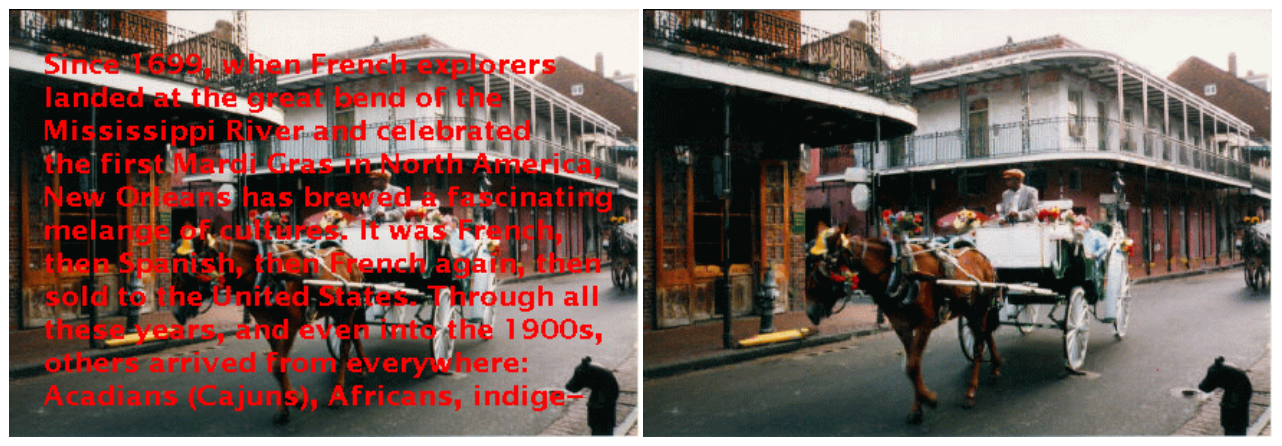
\includegraphics[width=\linewidth]{../thesis/Images/inpainting_bertalmio.png}
            \caption{Example for an application of inpainting in image
            restoration~\cite{bertalmio00}}
        \end{figure}
    \end{frame}

    \begin{frame}[t]
        \frametitle{What is inpainting\dots}
        \begin{itemize}[<+-|alert@+>]
            \item Restoration technique (antique paintings, photographs)
            \item ``Filling in'' of areas without having to know the data in these regions
            \item Digital inpainting introduced around 2000 (e.g.~\cite{bertalmio00, masnou98}) 
        \end{itemize}
    \end{frame}


    \begin{frame}[t]
        \frametitle{\dots and why do we care?}
        \begin{block}{Image Compression}<+->\ \\
            Inpainting based image compression methods are already able to outperform traditional
            codecs like JPEG for high compression rates 
        \end{block}
        \visible<2-> {
            \begin{figure}
                \centering
                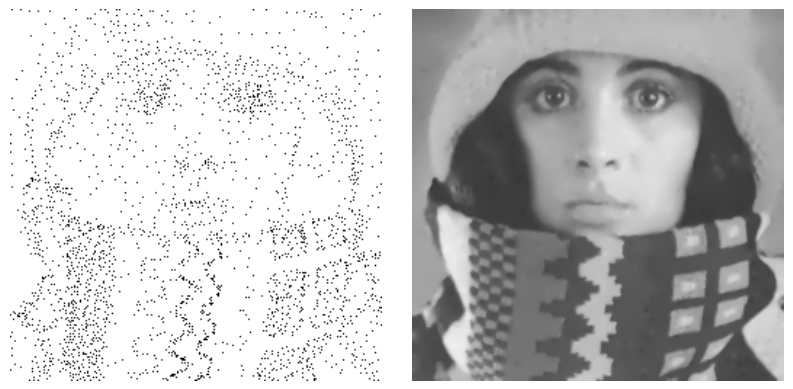
\includegraphics[width=0.85\textheight]{../thesis/Images/pde_example.png}
            \caption{Mask and respective reconstruction~\cite{hoeltgen12}}
            \end{figure}
        }
    \end{frame}


    \begin{frame}[t]
        \frametitle{Problem description}
        \begin{itemize}[<+-|alert@+>]
            \item Choosing optimal seed points for PDE-based inpainting is not trivial
            \item Many different approaches (semantic, tree-based, analytic, \dots)
            \item \textbf{Semantic:} Image features as seed points (edges/corners)
            \item Edge-based methods successful~\cite{mainberger10}
            \item Corners as seed points barely explored
        \end{itemize}
    \end{frame}

    \section{Previous Work}
    \begin{frame}[t]
        \frametitle{Previous Work}
        \textit{PDE-based inpainting using corner information~\cite{zimmer07}}\nobreak
        \begin{itemize}[<+-|alert@+>]
            \item Examined how well images can be compressed using only corners
            \item Masks as small neighbourhoods around important corners
            \item Interleaving mean curvature motion (MCM) and edge-enhancing diffusion
                (EED) for reconstruction
        \end{itemize}     
    \end{frame}

    \begin{frame}[t]
        \frametitle{Previous Work}
        \begin{figure}
            \centering
            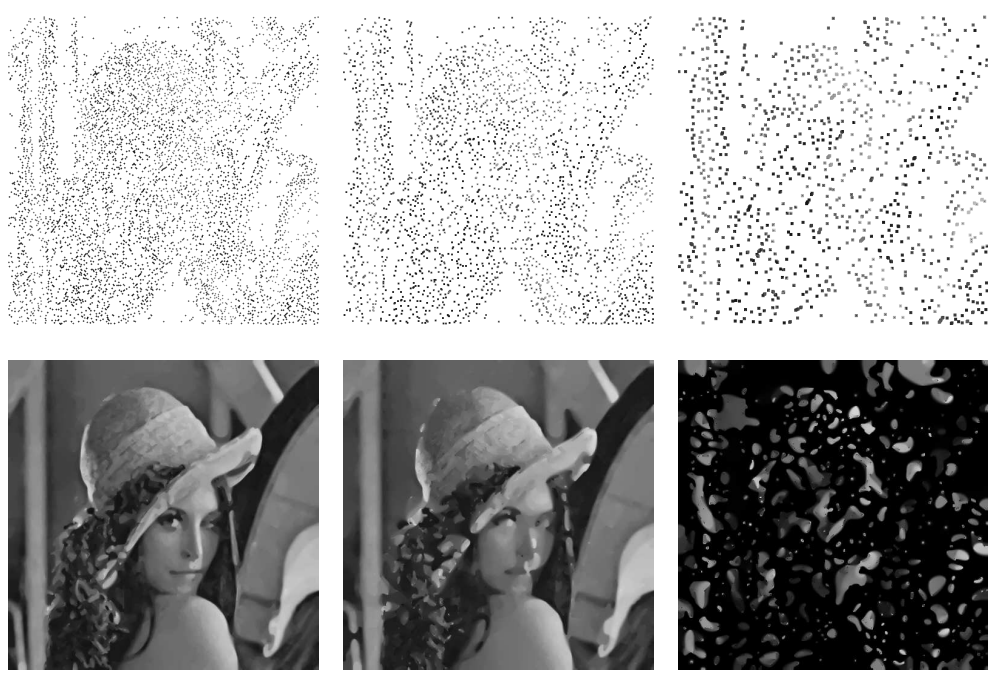
\includegraphics[width=\textheight]{../thesis/Images/zimmer_result.png}
            \caption{Reconstruction from corner regions of different sizes~\cite{zimmer07}}
        \end{figure}
    \end{frame}

    \begin{frame}[t]
        \frametitle{Previous Work}
        \textbf{Criticism:}
        \begin{itemize}[<+-|alert@+>]
            \item Inaccurate corner localisation
            \item Small masks might not capture the actual corners
            \item MCM not well suited for inpainting
        \end{itemize}
        \visible<+->{\textbf{Modifications:}}
        \begin{itemize}[]
            \item<4-|alert@4> Larger corner regions to capture displaced corners
            \item<+-|alert@+> Adapted thresholding
            \item<+-|alert@+> Pure EED inpainting
        \end{itemize}
    \end{frame}


    \section{Corner Regions + Localisation}
    \begin{frame}[t]
        \frametitle{Corner Detection based on the Structure Tensor}
        \visible<1,2,4->{
        \begin{itemize}
                \item<1-|alert@1> Structure tensor averages directional information in the
                    surrounding region
                    \[ J_\rho = K_\rho * (\nabla u_\sigma\nabla u_\sigma^\top) \]
                \item<2-|alert@2> Corner detection based on eigenvalues $\lambda_1, \lambda_2$
                \item<4-|alert@4> Förstner-Harris measure:
                    \[ \frac{\det{J_\rho}}{\tr{J_\rho}} = \frac{\lambda_1\lambda_2}{\lambda_1 + \lambda_2} > T\]
                \item<5-|alert@5> Local maxima marked as corners
            \end{itemize} 
        } 
        \only<3> {
            \vspace{-5cm}
            \begin{figure}
                \centering
                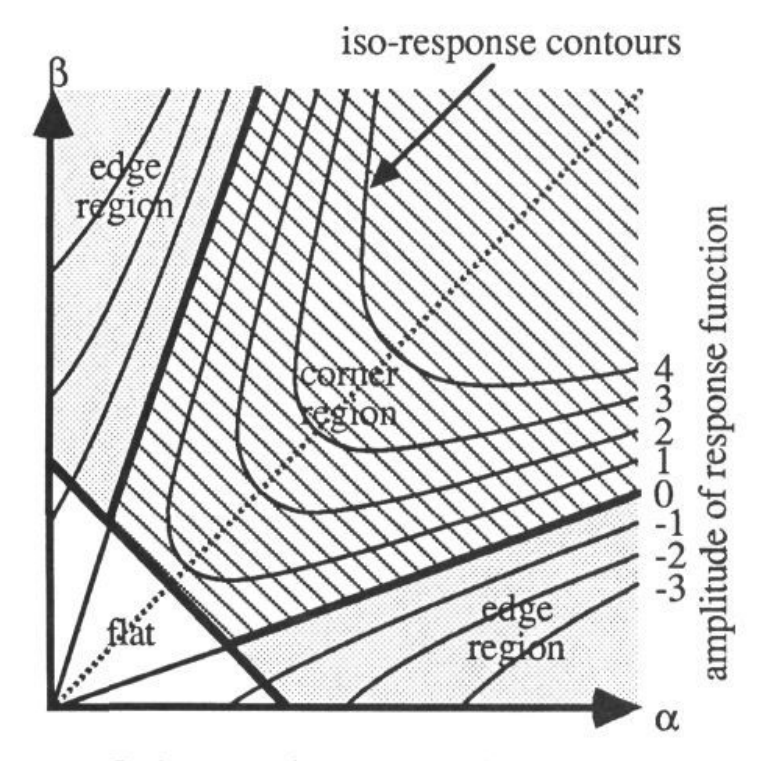
\includegraphics[height=0.7\textheight]{../thesis/Images/structure_tensor.png}
                \caption{Visualization of relation between eigenvalues of structure tensor~\cite{harris88}}
            \end{figure}
        }
    \end{frame}
    
    \begin{frame}[t]
        \frametitle{Effect of Integration Scale}
        \visible<1,2,4-> {\begin{itemize}
            \item<+-|alert@+> Increases uncertainty in localisation
            \item<+-|alert@+> Detected position might not align with actual position
            \item<4-|alert@4> Reconstruction errors 
            \item<5-|alert@5> Increasing integration scale to restrict amount of mask pixels not viable (as in
                \cite{zimmer07})
    \end{itemize}}
        \only<3>{
            \vspace{-3cm}
            \begin{figure}[htpb]
            \centering
            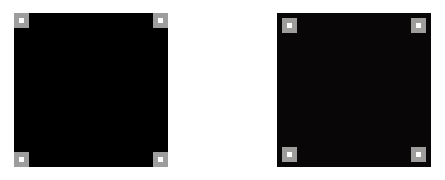
\includegraphics[width=\textheight]{images/mask_inacc.png}
            \caption{Corner regions similar to approach of~\cite{zimmer07} for different
            integration scales. \textbf{Left:} $\rho=2$ \textbf{Right:} $\rho=4$}
    \end{figure}}
    \end{frame}

    \begin{frame}[t]
        \frametitle{Choosing the Mask Radius}
        \begin{figure}[htpb]
            \centering
            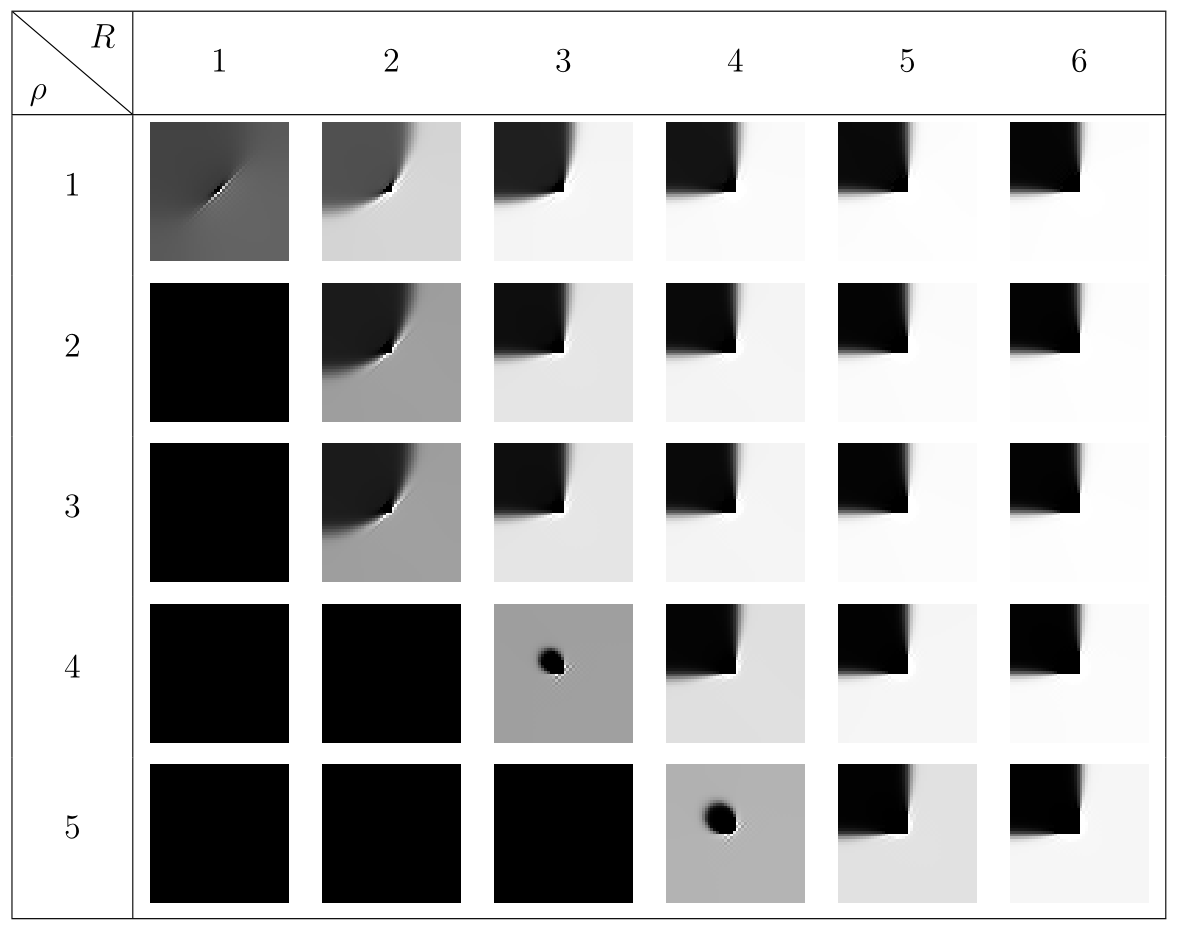
\includegraphics[width=0.7\linewidth]{images/matrix_inpaint.png}
            \caption{Matrix containing reconstruction results for different combinations of
            integration scale and mask radius}
        \end{figure} 
    \end{frame}

    \begin{frame}
        \frametitle{Choosing the Mask Radius}
        \begin{figure}[htpb]
            \centering
            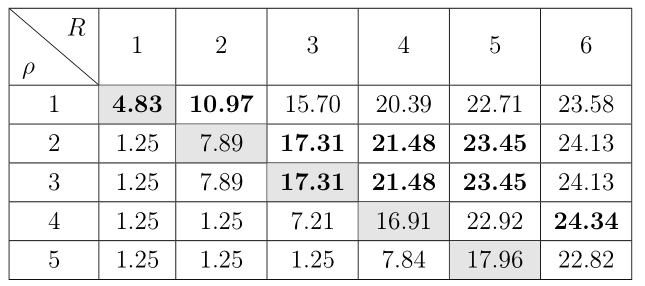
\includegraphics[width=0.7\linewidth]{images/psnr_mask.png}
            \caption{PSNR Values for reconstructed images from previous slide}
        \end{figure} 
    \end{frame}

    \begin{frame}[t]
        \frametitle{Choosing the Mask Radius}
        Results:
        \begin{itemize}[<+-|alert@+>]
            \item Experiments suggest choosing mask radius at least as large as integration
                scale
            \item Loss of information for too small radii
        \end{itemize}
    \end{frame}

    \section{Additional Modifications}
    \begin{frame}[t]
        \frametitle{Percentile Thresholding}
        \begin{block}{Problem}<+->\ \\
            Amount of corners varying on input image with fixed threshold\\
            Makes it hard to reliably produce masks of the same size
        \end{block}
        \begin{block}{Remedy}<+->\ \\
            Use so called percentile on cornerness map to filter out a certain percentage of
            corners
        \end{block}
        \begin{block}{Alternative}<+->\ \\
            Instead of filtering out percentage of corners, calculate upper bound for number of
            corners such that only a certain percentage of \textit{pixels} is kept.
        \end{block}
    \end{frame}  

    \begin{frame}[t]
        \frametitle{Percentile Thresholding}
        \begin{figure}[htpb]
            \centering
            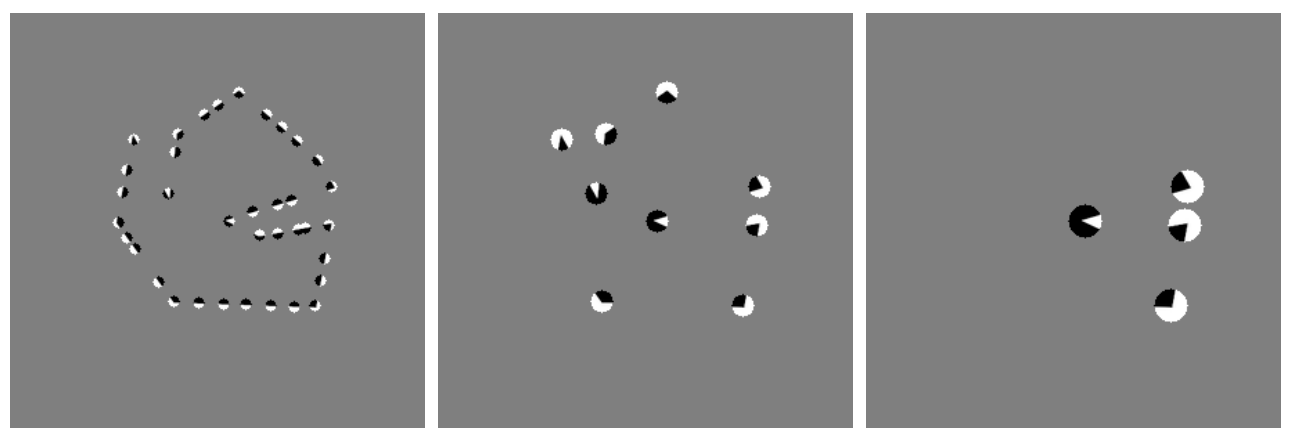
\includegraphics[width=\linewidth]{images/tppt.png}
            \caption{Mask of similar size for different radii. Upper bound: 2\% of total pixels.
            Actual sizes: 1.95\%, 1.97\%, 1.96\%}
        \end{figure}
    \end{frame}

     \begin{frame}[t]
        \frametitle{Non-maximum Suppression}
        \begin{block}{Observation}<+->\ \\
            Corner regions tend to overlap a lot, especially in textured regions\\
            Results in poorly distributed inpainting mask
        \end{block} 
        \begin{block}{Possible Remedy}<+->\ \\
            Discard corners already covered by a `better' corner 
        \end{block}
     \end{frame} 

    \begin{frame}[t]
        \frametitle{Non-maximum Suppression}
        \begin{figure}[htpb]
            \centering
            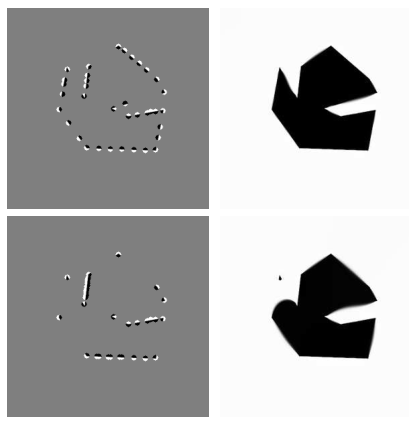
\includegraphics[height=0.5\linewidth]{images/cnms2.png}
            \caption{Effect of CNMS on the distribution of corner regions across the image.
            Parameters: $\sigma=1,\rho=1,R=4,q=0.02$. \textbf{Top:} CNMS, \textbf{Bottom:} no CNMS}
        \end{figure} 
    \end{frame}

    \section{Reconstruction}
    \begin{frame}[t]
        \frametitle{Reconstruction}
        \visible<1-3,5->{\begin{itemize}
            \item<+-|alert@+>Reconstruction based on edge-enhancing diffusion
            \item<+-|alert@+>Type of anisotropic diffusion governed by PDE
                \[ \partial_t u = \text{div}(g(\nabla u_\sigma\nabla u_\sigma^\top)\nabla u) \]
            \item<+-|alert@+>Originally meant for denoising
            \item<5-|alert@5>Considered one of the best inpainting operators~\cite{schmaltz14}
    \end{itemize}}
        \only<4>{
            \vspace{-4.5cm}
            \begin{figure}[htpb]
                \centering
                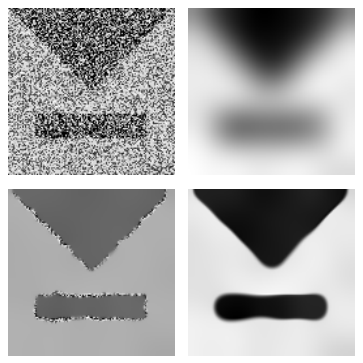
\includegraphics[height=0.6\textheight]{../thesis/Images/diff_examples.png}
                \caption{ \textbf{Top Left:} Original image, \textbf{Top Right:} Homogeneous
                Diffusion, \textbf{Bottom Left:} Nonlinear isotropic diffusion, \textbf{Bottom
            Right:} EED}
            \end{figure}
        }
    \end{frame}

    \begin{frame}[t]
        \frametitle{Reconstruction}
        \begin{figure}[htpb]
            \centering
            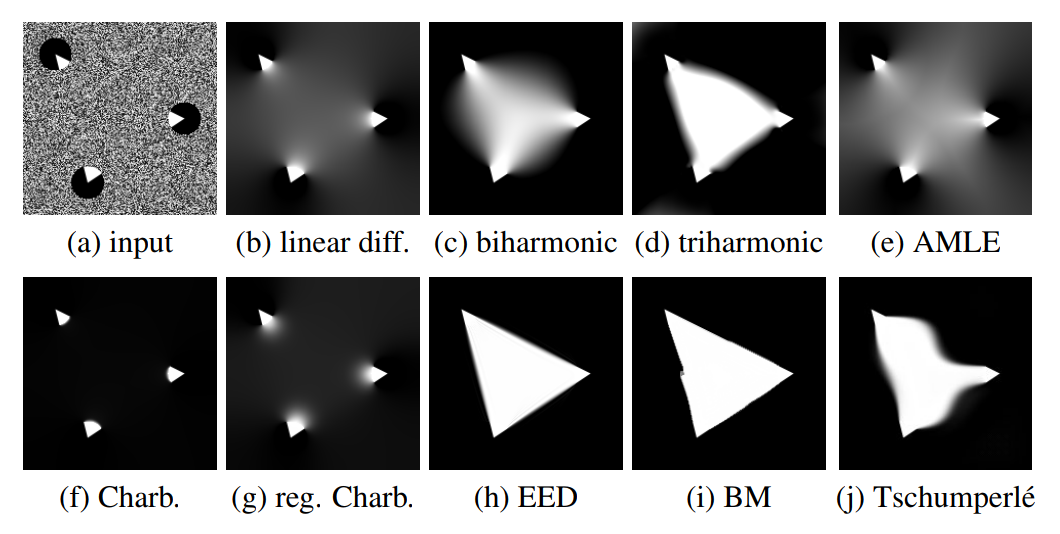
\includegraphics[width=0.8\linewidth]{../thesis/Images/diffops_compare.png}
            \caption{Comparison of inpainting operators~\cite{schmaltz14}}
        \end{figure}
    \end{frame}

    \section{Results}
    \begin{frame}
        \frametitle{Results}
        \begin{figure}[htpb]
            \centering
            
\includegraphics[width=0.3\linewidth]{../images/binary/abstract1_small.png}
            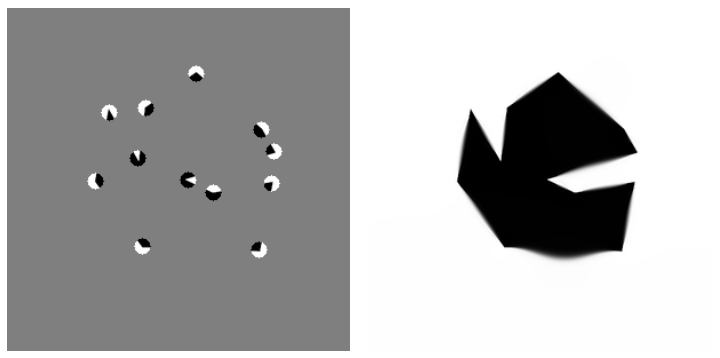
\includegraphics[width=0.6\linewidth]{images/abstract2.png}
            \caption{ \textbf{Left:} Original image, \textbf{Middle:} Inpainting mask
                ($\sigma=1,\rho=1,R=7,q=0.02$) 1.99\% of all pixels, \textbf{Right:} Reconstruction
            ($\sigma=2,\lambda=0.1,\alpha=0.49,\gamma=1, PSNR: 18.35$) }
        \end{figure}        
    \end{frame}

    \begin{frame}
        \frametitle{Results}
        \begin{figure}[htpb]
            \centering
            
\includegraphics[width=0.3\linewidth]{../images/binary/abstract1_small.png}
            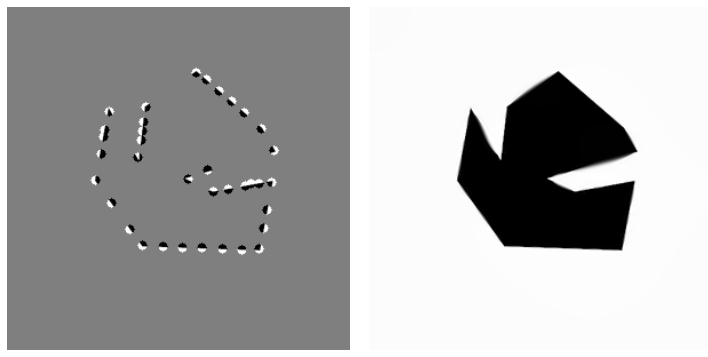
\includegraphics[width=0.6\linewidth]{images/abstract.png}
            \caption{ \textbf{Left:} Original image, \textbf{Middle:} Inpainting mask
                ($\sigma=1,\rho=1,R=4,q=0.02$) 1.96\% of all pixels, \textbf{Right:} Reconstruction
            ($\sigma=2,\lambda=0.1,\alpha=0.49,\gamma=1, PSNR: 31.45$) }
        \end{figure}        
    \end{frame}

    \begin{frame}
        \frametitle{Results}
        \begin{figure}[htpb]
            \centering
            
\includegraphics[width=0.3\linewidth]{../images/binary/cat.png}
            
\includegraphics[width=0.6\linewidth]{images/cat.png}
            \caption{ \textbf{Left:} Original image, \textbf{Middle:} Inpainting mask
                ($\sigma=1,\rho=1,R=10$) 4.74\% of all pixels, \textbf{Right:} Reconstruction
            ($\sigma=2,\lambda=0.2,\alpha=0.49,\gamma=1, PSNR: 18.35$) }
        \end{figure}
    \end{frame}

    \begin{frame}
        \frametitle{Results}
        \begin{figure}[htpb]
            \centering
            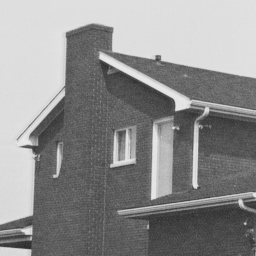
\includegraphics[width=0.3\linewidth]{../images/grey/house.png}
            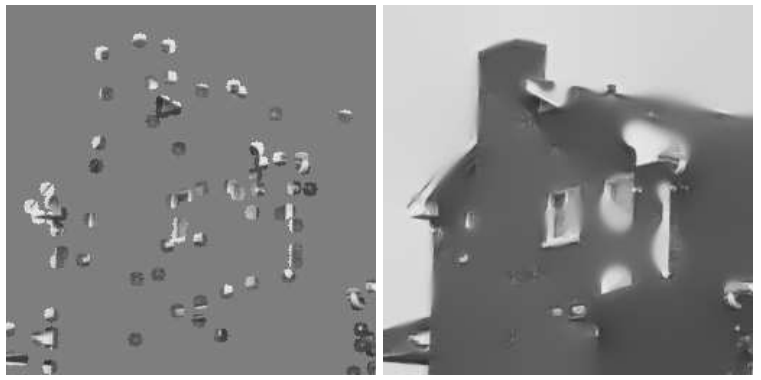
\includegraphics[width=0.6\linewidth]{images/house.png}
            \caption{ \textbf{Left:} Original image, \textbf{Middle:} Inpainting mask ($\sigma=1,
            \rho=1, R=5, q=0.1$) 9.23\% of all pixels, \textbf{Right:} Reconstruction
            ($\sigma=2,\lambda=0.4,\alpha=0.49,\gamma=1, PSNR: 21.11)$} 
        \end{figure}
    \end{frame}


    \begin{frame}
        \frametitle{Results}
        \begin{figure}[htpb]
            \centering
            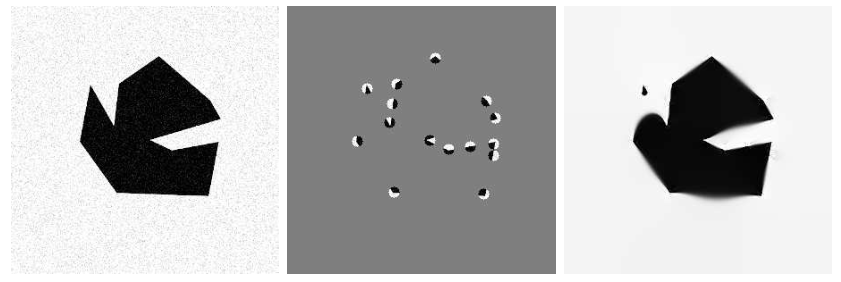
\includegraphics[width=\linewidth]{images/less_noise.png}
            \caption{ \textbf{Left:} Original image, \textbf{Middle:} Inpainting mask ($\sigma=1.5,
            \rho=2, R=6, q=0.02$) 1.88\% of all pixels, \textbf{Right:} Reconstruction
            ($\sigma=2,\lambda=0.2,\alpha=0.49,\gamma=1, PSNR: 20.74)$} 
        \end{figure}
    \end{frame}

    \begin{frame}
        \frametitle{Results}
        \begin{figure}[htpb]
            \centering
            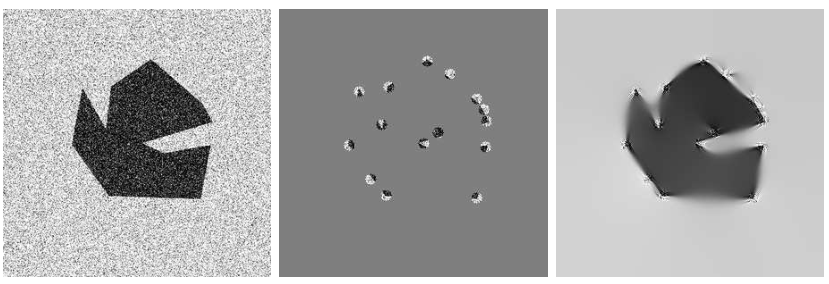
\includegraphics[width=\linewidth]{images/more_noise.png}
            \caption{ \textbf{Left:} Original image, \textbf{Middle:} Inpainting mask ($\sigma=1.5,
            \rho=2, R=6, q=0.02$) 1.88\% of all pixels, \textbf{Right:} Reconstruction
            ($\sigma=2,\lambda=0.2,\alpha=0.49,\gamma=1, PSNR: 16.25)$}
        \end{figure}
    \end{frame}

    \section{Conclusion}
    \begin{frame}[t]
        \frametitle{Conclusion}
        \begin{itemize}[<+-|alert@+>]
            \item Choose mask radius at least as large as integration scale
            \item Fairly good results for binary images
            \item Struggles with textured images
            \item Corners are fairly seldom 
        \end{itemize}
        
    \end{frame}

    \begin{frame}
        \centering\huge{Any questions?}
    \end{frame}

    \begin{frame}
        \centering\huge{Thank you for your time!}
    \end{frame}

%~~~~~~~~~~~~~~~~~~~~~~~~~~~~~~~~~~~~References~~~~~~~~~~~~~~~~~~~~~~~~~~~~~~~~~~~~~~~~~~~
    \section{References}
    \begin{frame}[t, allowframebreaks]
        \frametitle{Bibliography}
        \bibliographystyle{apalike}
        \bibliography{../thesis/references.bib}
    \end{frame}

    \backupbegin
    \section*{Appendix}

    \begin{frame}
    \end{frame}
    \backupend

\end{document}
